% MiniDB 实验二（索引）实验报告
% 编译：xelatex report-exp2.tex（运行两次以生成目录）
\documentclass[11pt,a4paper]{ctexart}

\usepackage[margin=2.4cm]{geometry}
\usepackage{booktabs}
\usepackage{tabularx}
\usepackage{array}
\usepackage{xcolor}
\usepackage{listings}
\usepackage{graphicx}
\usepackage{tikz}
\usetikzlibrary{positioning,calc}
\usepackage{amsmath}
\usepackage{enumitem}
\usepackage{caption}
\usepackage{float}
\usepackage{fancyhdr}
\usepackage[hidelinks]{hyperref}

\setlist{itemsep=2pt,topsep=4pt}
\setlength{\emergencystretch}{3em}
\captionsetup{font=small,labelfont=bf}
\renewcommand{\arraystretch}{1.15}

\definecolor{codebg}{RGB}{247,247,247}
\definecolor{codecomment}{RGB}{0,110,0}
\definecolor{codekw}{RGB}{0,0,160}
\definecolor{todo}{RGB}{200,0,0}

% 待填写的内容用红色标出，定稿前全部替换
\newcommand{\TODO}[1]{\textcolor{todo}{【待填写：#1】}}

\lstset{
  basicstyle=\ttfamily\footnotesize,
  backgroundcolor=\color{codebg},
  keywordstyle=\color{codekw}\bfseries,
  commentstyle=\color{codecomment},
  frame=single, rulecolor=\color{black!25},
  breaklines=true, columns=fullflexible, keepspaces=true,
  showstringspaces=false, tabsize=2,
  numbers=left, numberstyle=\tiny\color{black!50}, xleftmargin=2em,
}
\lstdefinestyle{plain}{numbers=none,xleftmargin=0pt,keywordstyle=,commentstyle=}
\lstdefinestyle{wide}{style=plain,basicstyle=\ttfamily\scriptsize}

\pagestyle{fancy}
\fancyhf{}
\fancyhead[L]{\small 数据库系统实验二：索引}
\fancyhead[R]{\small MiniDB 实验报告}
\fancyfoot[C]{\thepage}

\newcommand{\code}[1]{\texttt{#1}}

\begin{document}

\begin{titlepage}
  \centering
  \vspace*{3cm}
  {\Huge\bfseries 数据库系统实验报告\par}
  \vspace{1cm}
  {\LARGE 实验 02：索引\par}
  \vspace{0.6cm}
  {\large MiniDB —— 外存 B+ 树索引的建立、维护与查找\par}
  \vspace{3cm}
  \begin{tabular}{rl}
    课程名称： & 数据库系统 \\[4pt]
    小组成员： & 任勇宁，彭文博，边宇晗，章国文，张睿涵 \\[4pt]
    提交日期： & 2026 年 11 月 11 日 \\
  \end{tabular}
  \vfill
  {\small 代码仓库：\url{https://github.com/renyongning/MiniDB}\par}
\end{titlepage}

\tableofcontents
\newpage

% ================================================================== 1
\section{实验分工安排}

\begin{table}[H]
  \centering
  \caption{小组分工}
  \begin{tabularx}{\textwidth}{l X}
    \toprule
    成员 & 负责内容 \\
    \midrule
    任勇宁 & \TODO{本次实验负责内容} \\
    彭文博 & \TODO{本次实验负责内容} \\
    边宇晗 & \TODO{本次实验负责内容} \\
    章国文 & \TODO{本次实验负责内容} \\
    张睿涵 & \TODO{本次实验负责内容} \\
    \bottomrule
  \end{tabularx}
\end{table}

% ================================================================== 2
\section{实验环境}

\begin{table}[H]
  \centering
  \caption{开发与测试环境}
  \begin{tabularx}{\textwidth}{l X}
    \toprule
    项目 & 说明 \\
    \midrule
    编程语言 & C++20，与实验一相同 \\
    构建工具 & CMake $\geq$ 3.16 \\
    第三方依赖 & 无 \\
    测试平台 & Ubuntu 24.04.4 LTS（Linux 7.0，x86-64），AMD EPYC 9654，GCC 12.4.0，CMake 4.3.0，Release 构建 \\
    验收平台 & \TODO{验收时使用的操作系统与编译器版本} \\
    \bottomrule
  \end{tabularx}
\end{table}

页大小为 8 KB。测试默认使用 1024 帧（8 MB）缓冲池，演示脚本和验收程序使用 16 帧（128 KB）缓冲池。测试数据为课程提供的 TPC-H 数据：\code{supplier} 1 万行、\code{orders} 150 万行、\code{lineitem} 600 万行。

% ================================================================== 3
\section{实验设计与实现}

本实验在实验一的存储引擎上实现 B+ 树索引。B+ 树同时支持等值查询和范围查询，是三种候选结构中适用面最广的一种。

\subsection{总体结构}

\begin{table}[H]
  \centering
  \caption{索引相关模块}
  \begin{tabularx}{\textwidth}{l X}
    \toprule
    模块 & 职责 \\
    \midrule
    \code{src/index/bplus\_tree.*} & B+ 树：索引文件与节点页格式、查找、插入、删除、范围扫描、批量建树、结构校验与绘图。只依赖缓冲池和磁盘管理器 \\
    \code{src/db/index.cpp} & \code{CREATE/DROP INDEX}、打开数据库时加载索引、增删改后的索引维护 \\
    \code{src/db/database.cpp} & 执行器。\code{FindRows} 为 \code{SELECT/UPDATE/DELETE} 选择索引扫描或堆扫描 \\
    \code{src/db/pragma.cpp} & 索引的查看、校验与绘图命令 \\
    \bottomrule
  \end{tabularx}
\end{table}

每个索引对应数据库目录下 \code{indexes/} 中的一个 \code{.idx} 文件。打开数据库时逐个加载索引，并核对其中记录的表 ID、列序号、键类型和长度与系统目录一致。

\subsection{索引文件与页格式}

索引文件沿用实验一的文件头、32 字节通用页头、CRC32C 校验和以及按区（64 页）扩展的方式。

\begin{table}[H]
  \centering
  \caption{索引文件的页}
  \begin{tabularx}{\textwidth}{l l X}
    \toprule
    页号 & 页类型 & 内容 \\
    \midrule
    0 & 文件头 & 与数据文件相同，文件类型为 \code{kIndex} \\
    1 & \code{kBtreeMeta} & 格式版本、列序号、键类型与长度、根页号、下一个未用页号、空闲页链表头、索引项总数、索引名与表名 \\
    2 起 & \code{kBtreeLeaf} / \code{kBtreeInternal} & 树节点 \\
    2 起 & \code{kBtreeFree} & 合并后释放的页，页内存放下一个空闲页号，构成链表 \\
    \bottomrule
  \end{tabularx}
\end{table}

节点页在通用页头之后是 32 字节的节点头，随后是定长槽位（图~\ref{fig:node}）。

\begin{figure}[H]
  \centering
  \begin{tikzpicture}[font=\small, box/.style={draw, minimum height=0.8cm, inner sep=2pt}]
    \node[box, minimum width=2.2cm, fill=black!8] (h) {通用页头};
    \node[box, minimum width=1.3cm, right=0pt of h] (c) {项数};
    \node[box, minimum width=1.8cm, right=0pt of c] (n) {下一叶};
    \node[box, minimum width=2.0cm, right=0pt of n] (f) {最左孩子};
    \node[box, minimum width=1.2cm, right=0pt of f, fill=black!4] (r) {保留};
    \node[box, minimum width=2.6cm, right=0pt of r, fill=blue!8] (s0) {槽位 0};
    \node[box, minimum width=2.6cm, right=0pt of s0, fill=blue!8] (s1) {槽位 1};
    \node[box, minimum width=1.2cm, right=0pt of s1] (d) {$\cdots$};
    \node[below=2pt of h] {0--31};
    \node[below=2pt of c] {32};
    \node[below=2pt of n] {36};
    \node[below=2pt of f] {40};
    \node[below=2pt of s0] {64};
    \node[box, minimum width=3.4cm, below=1.5cm of n, fill=blue!8] (k) {键};
    \node[box, minimum width=2.4cm, right=0pt of k, fill=blue!8] (rid) {RID（6 字节）};
    \node[box, minimum width=3.4cm, right=0pt of rid, fill=blue!8] (ch) {右孩子页号（4 字节）};
    \draw[dashed] (s0.south west) -- (k.north west);
    \draw[dashed] (s0.south east) -- (ch.north east);
    \node[below=2pt of k] {整型 8 字节；字符型 $2+n$ 字节};
    \node[below=2pt of ch] {仅内部节点};
  \end{tikzpicture}
  \caption{节点页布局}
  \label{fig:node}
\end{figure}

\begin{itemize}
  \item 整型键存为 8 字节有符号整数。字符型键存为 2 字节长度加内容，槽位宽度由列的声明长度 $n$ 决定。
  \item 内部节点的第 $i$ 个槽位保存第 $i$ 个分隔键及其右侧的孩子，最左侧的孩子保存在节点头中。在内部节点加入或移除一个分隔键及其右孩子，对应插入或删除一个槽位。
  \item 节点容量为 $\lfloor (8192-64)/(\text{键宽}+6+4) \rfloor$ 向下取偶：整型键 450，\code{CHAR(25)} 218，\code{CHAR(15)} 300。非根节点至少半满。
\end{itemize}

\subsection{键的顺序}

索引为非唯一索引，索引项按（键，RID）排序，键相同的项按记录地址排序。重复键因此可以跨越多个叶子，删除时可以精确定位到单个索引项，内部节点的分隔键也采用同一顺序。

键的比较与 SQL 层一致：整数按 64 位整数比较；字符串按字节字典序比较，尾部空白不参与比较，\code{CHAR(n)} 列补齐的空格不影响匹配。\code{NULL} 不进入索引。

\subsection{查找与范围扫描}

点定位从根开始，在每层节点内二分确定要进入的孩子，直到叶子。叶子通过“下一叶”页号连成链表，范围扫描沿链表进行。

\code{Scan(op, key, visitor)} 支持 $=$、$<$、$\leq$、$>$、$\geq$、$\neq$ 六种比较。$=$、$>$、$\geq$ 从键所在的叶子开始，其余从最左叶子开始；$=$、$<$、$\leq$ 在遇到第一个大于键的项时结束。访问函数返回 \code{false} 时扫描提前结束，\code{LIMIT} 据此实现。

\subsection{插入与删除}

\paragraph{插入}自顶向下递归到叶子，在叶内二分定位后插入。节点项数超过容量时分裂，上半部分移入新分配的右兄弟：叶子分裂时中间项保留在右兄弟并复制为父节点的分隔键，右兄弟接入叶子链；内部节点分裂时中间的分隔键上移到父节点。分裂沿返回路径向上传播，到达根时生成新根，树高加一。

\paragraph{删除}按（键，RID）定位并从叶子移除。节点少于半满时由父节点调整：优先从左兄弟借一项，其次从右兄弟借一项，两者都不富余时与兄弟合并，父节点移除对应的分隔键，释放的页加入空闲页链表。调整沿路径向上传播；内部根节点只剩一个孩子时，由该孩子接任根，树高减一。

插入和删除只写回内容发生变化的节点。分配新页时优先复用空闲页链表中的页。

\subsection{内外存数据交换}

索引页全部通过实验一的 \code{BufferPool} 读写。读页时页从磁盘调入缓冲帧并校验 CRC；写页时在缓冲帧中修改并标记为脏页，由 CLOCK 淘汰或 \code{flush} 写回磁盘。

\paragraph{节点工作副本}分裂、借位与合并需要同时操作父节点、当前节点和兄弟节点。\code{Node} 是一页的工作副本：读节点时复制页的字节并立即释放缓冲帧，修改在副本上进行，写节点时再申请缓冲帧写回。树在任意时刻最多占用一个缓冲帧，2 帧的缓冲池即可完成全部操作；范围扫描回表读取堆页时，索引页不占用缓冲帧。

\paragraph{页内字节操作}工作副本保持页的磁盘编码。查找直接比较槽位中的字节，插入和删除是一次 \code{memmove}，分裂与合并是整段槽位的复制；只有分隔键和扫描结果需要解码为值。性能分析显示，节点访问是插入路径上的主要 CPU 开销，这一设计使其不再包含解码和内存分配。

\subsection{索引的建立}

\code{CREATE INDEX} 采用外部归并排序与自底向上装载，这也是 PostgreSQL 和 InnoDB 建立 B 树索引的方式。建树所需内存由排序预算决定，与表的大小无关。

\begin{enumerate}
  \item \textbf{生成有序段}。扫描堆表，把每行的（键，RID）编码为紧凑记录，写入固定大小的排序缓冲（默认 64 MB，可用 \code{PRAGMA index\_sort\_memory} 设置）。缓冲写满时排序，并作为一个有序段追加到临时文件。
  \item \textbf{多路归并}。用小顶堆归并各有序段，每段占用一个读缓冲（排序预算的八分之一，8 KB 至 64 KB）。归并路数等于预算可容纳的读缓冲数；有序段多于该路数时，先将相邻的段归并为更长的段，直到一次归并可以完成。
  \item \textbf{自底向上装载}。归并输出的有序流依次填充叶子页，页填满后写出，并把页号和最小项交给上一层；上一层按同样方式填充。每层在内存中只保留一个正在填充的节点。
\end{enumerate}

总项数在归并前已知，各层的节点数和每个节点的项数据此预先确定并均匀分配，每个节点预留八分之一空间，所有非根节点满足半满约束。数据量小于排序预算时直接在内存排序，不产生临时文件。建树写入 \code{.building} 文件，完成并刷盘后改名为 \code{.idx}。

\subsection{与 SQL 层的衔接}

\paragraph{行定位}\code{SELECT}、\code{UPDATE}、\code{DELETE} 的 \code{WHERE} 条件由 \code{Database::FindRows} 统一处理：条件列上有索引时沿索引扫描并按 RID 回表，否则顺序扫描堆表。$\neq$ 条件命中绝大多数行，采用堆扫描。使用索引时，语句的结果消息显示 \code{INDEX SCAN 索引名}。\code{UPDATE} 和 \code{DELETE} 先收集全部命中的行再修改，被修改的索引项不会在同一次扫描中再次命中。

\paragraph{索引维护}\code{INSERT} 和 \code{COPY} 在堆表插入后向该表的每个索引插入新项；\code{DELETE} 删除对应的项；\code{UPDATE} 对键值发生变化的索引执行一次删除和一次插入。堆表的行在变长迁移后保持原 RID，索引中的记录地址始终有效。\code{DROP TABLE} 同时删除该表的索引。

\subsection{模块接口}

\begin{lstlisting}[language=C++,style=plain]
class BPlusTree {
 public:
  static Result<std::unique_ptr<BPlusTree>> Create(
      BufferPool& pool, const std::string& path, const IndexMetadata& metadata);
  static Result<std::unique_ptr<BPlusTree>> Open(BufferPool& pool,
                                                 const std::string& path);

  // Builds an empty tree from entries added in any order (CREATE INDEX).
  class BulkLoader {
   public:
    explicit BulkLoader(BPlusTree& tree,
                        size_t memory_bytes = kDefaultSortMemory);
    Status Add(const Value& key, RID rid);
    Status Finish();
  };

  Status Insert(const Value& key, RID rid);
  Status Erase(const Value& key, RID rid);
  // Visits matching entries in key order; the visitor returns false to stop.
  Status Scan(CompareOp op, const Value& key,
              const std::function<bool(const IndexEntry&)>& visitor);
  Result<std::vector<RID>> Find(const Value& key);

  Result<IndexStats> Validate();  // checks every invariant of the whole tree
  Result<std::string> Draw(size_t max_nodes = 128);  // indented text
  Result<std::string> Dot(size_t max_nodes = 128);   // Graphviz source
};
\end{lstlisting}

\begin{itemize}
  \item 树的接口只涉及键和 RID，与表、元组和 SQL 无关，可以独立测试。数据地址即实验一堆表的 RID（页号与槽号）。
  \item 操作返回 \code{Status} 或 \code{Result<T>}，与存储层一致。从磁盘读入的元数据、页类型、项数和页号都经过检查，不一致时返回 \code{kCorruption}。
  \item \code{Scan} 通过访问函数逐项返回结果，范围查询无需物化结果集。
  \item \code{Validate} 遍历整棵树，检查键有序、分隔键范围、半满约束、叶子深度一致、叶子链完整、项数与元数据一致、空闲页链表与在用页不相交、所有页可达。
\end{itemize}

% ================================================================== 4
\section{使用手册}

\subsection{编译与启动}

\begin{lstlisting}[language=bash,style=plain]
cmake -S . -B build -DCMAKE_BUILD_TYPE=Release
cmake --build build -j
./build/minidb_shell --db /tmp/demo_db
\end{lstlisting}

\subsection{索引相关的 SQL}

\begin{lstlisting}[language=SQL,style=plain]
CREATE INDEX [IF NOT EXISTS] index_name ON table_name(column);
DROP INDEX [IF EXISTS] index_name;

SELECT ... FROM t WHERE column op value [LIMIT n];
UPDATE t SET ... WHERE column op value;
DELETE FROM t WHERE column op value;
\end{lstlisting}

索引为单列非唯一索引，列类型为 \code{INTEGER}、\code{BIGINT}、\code{CHAR(n)} 或 \code{VARCHAR(n)}（$n \leq 4000$）。一个表可以建立多个索引。\code{WHERE} 列上有索引时自动使用。

\subsection{查看与校验}

\begin{table}[H]
  \centering
  \caption{索引相关的 PRAGMA}
  \begin{tabularx}{\textwidth}{l X}
    \toprule
    命令 & 作用 \\
    \midrule
    \code{PRAGMA indexes[(table)]} & 列出索引及其所属表、列、类型和项数 \\
    \code{PRAGMA index\_check(index)} & 校验整棵树，输出项数、树高、节点数、叶子数、空闲页数、节点容量和根页号 \\
    \code{PRAGMA index\_tree(index)} & 以缩进文本绘制树：节点页号、项数、前几个键及 RID、叶子链 \\
    \code{PRAGMA index\_dot(index)} & 输出 Graphviz DOT 图源 \\
    \code{PRAGMA index\_sort\_memory [= KB]} & 查看或设置建索引的排序内存预算 \\
    \code{PRAGMA buffer\_stats} & 缓冲池的命中、缺页、淘汰和写回次数 \\
    \bottomrule
  \end{tabularx}
\end{table}

\subsection{演示与验收程序}

\begin{lstlisting}[language=bash,style=plain]
# 演示脚本：建两种类型的索引、绘制树、点查与范围查、增删改、校验、外部归并建树
./build/minidb_shell --db /tmp/demo_db --buffer 16 --file scripts/demo_index.txt

# 验收程序：supplier 上两种索引，重开后核对 20000 次点查找，范围查询与全表扫描对照
./build/minidb_verify_index_tpch test/tpc-h/supplier.tbl /tmp/verify_db
\end{lstlisting}

% ================================================================== 5
\section{测试方案和结果}

\subsection{测试方案}

\begin{table}[H]
  \centering
  \caption{测试内容}
  \begin{tabularx}{\textwidth}{l X}
    \toprule
    测试 & 内容 \\
    \midrule
    随机测试 & 1 万个整数项和 5 千个字符串项乱序插入、交错删除，键大量重复；每阶段校验全树，并将六种比较运算的扫描结果与参考集合比对；4 帧缓冲池，关闭重开后再比对 \\
    边界测试 & 容量为 2 的索引形成 5 层以上的树后全部删除；含 NUL 字节的字符串、超长键、类型不符的键；\code{BIGINT} 的极值和超过 $2^{53}$ 的相邻值 \\
    批量建树 & 三种节点容量（2、30、450）和多种数据规模，分别在内存排序和 2 KB 排序预算（上百个有序段、多趟归并）下建树，校验后继续增删 \\
    SQL 集成 & 建索引前后查询结果一致；\code{NULL}、\code{CHAR} 补齐、\code{LIMIT}、同列多个索引、\code{COPY}、重开、\code{DROP} \\
    增删改对照 & 16 条 \code{UPDATE/DELETE} 分别在有索引和无索引的相同表上执行，逐条比对表内容和索引项数 \\
    损坏检测 & 改写索引页的一个字节后，查找返回校验和错误 \\
    真实数据 & supplier 上两种类型的索引，重开后 2 万次点查找逐条核对；orders 与 lineitem 上的规模测试 \\
    \bottomrule
  \end{tabularx}
\end{table}

自动化测试在 Release 构建以及开启 AddressSanitizer 和 UndefinedBehaviorSanitizer 的构建下全部通过。

\begin{lstlisting}[style=plain]
    Start 1: minidb_integration
1/3 Test #1: minidb_integration ...............   Passed    0.11 sec
    Start 2: minidb_storage
2/3 Test #2: minidb_storage ...................   Passed    0.02 sec
    Start 3: minidb_index
3/3 Test #3: minidb_index .....................   Passed    1.31 sec
100% tests passed, 0 tests failed out of 3
Total Test time (real) =   1.45 sec
\end{lstlisting}

\subsection{supplier 上的两种索引}

在 \code{supplier}（1 万行）的 \code{s\_suppkey}（\code{INTEGER}）和 \code{s\_name}（\code{CHAR(25)}）上建立索引，使用 16 帧缓冲池。

\begin{table}[H]
  \centering
  \caption{supplier 两个索引的结构}
  \begin{tabular}{lrr}
    \toprule
    项目 & supplier\_key & supplier\_name \\
    \midrule
    索引列 & s\_suppkey & s\_name \\
    数据类型 & INTEGER & CHAR(25) \\
    索引项数 & 10000 & 10000 \\
    树高 & 2 & 2 \\
    节点总数 & 27 & 54 \\
    叶节点数 & 26 & 53 \\
    节点容量 & 450 & 218 \\
    结构校验 & ok & ok \\
    \bottomrule
  \end{tabular}
\end{table}

字符键较宽，每页容纳的项较少，叶子数相应增加。两棵树的结构见图~\ref{fig:key} 和图~\ref{fig:name}，图中画出前两个和后两个叶子。

\begin{figure}[H]
  \centering
  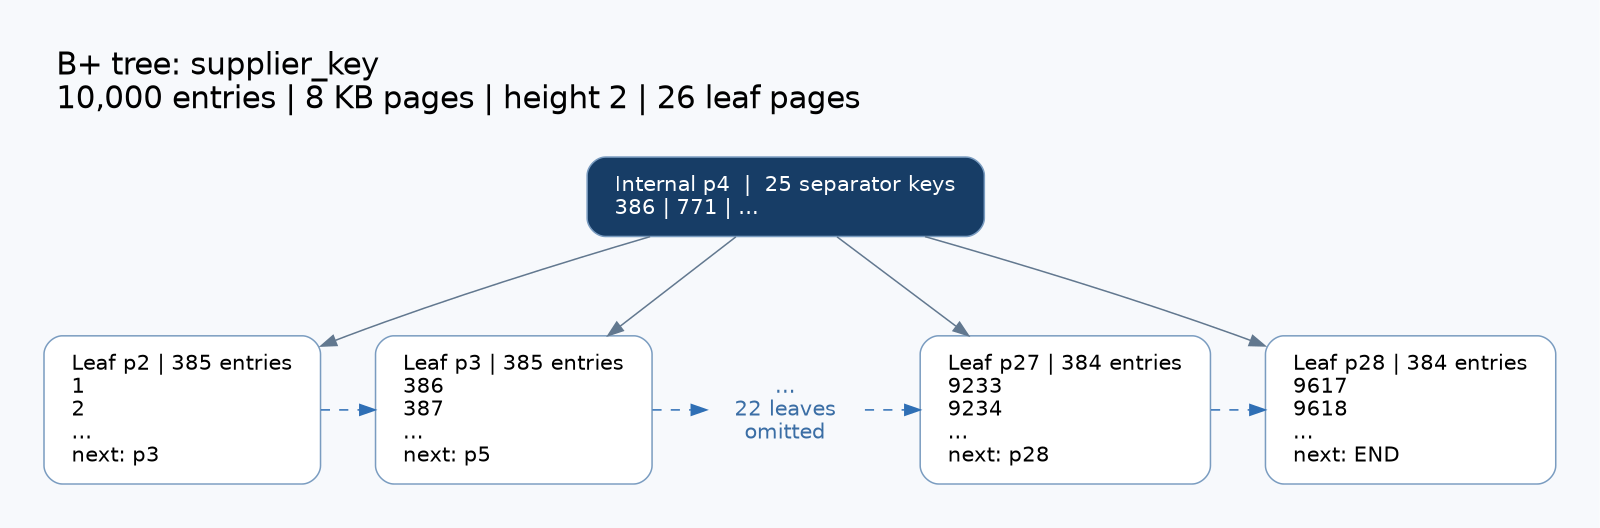
\includegraphics[width=\textwidth]{../exp2-evidence/supplier_key.png}
  \caption{supplier 整型索引的 B+ 树}
  \label{fig:key}
\end{figure}

\begin{figure}[H]
  \centering
  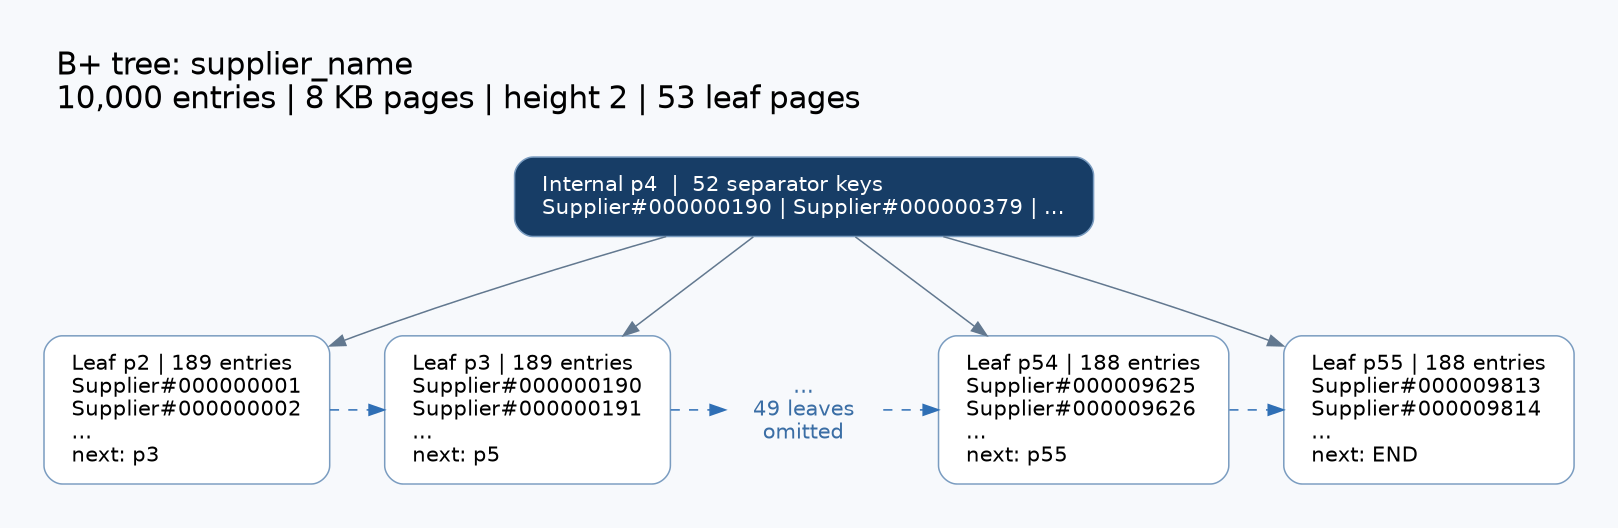
\includegraphics[width=\textwidth]{../exp2-evidence/supplier_name.png}
  \caption{supplier 字符索引的 B+ 树}
  \label{fig:name}
\end{figure}

关闭并重新打开数据库后，按两种键核对全部源记录，2 万次点查找全部一致；范围查询与全表扫描结果一致；增删改及再次重开后的核对全部通过。

\subsection{演示脚本输出}

以下输出摘自 \code{scripts/demo\_index.txt} 的运行结果。

\paragraph{建立索引与树图}两种类型的索引及整型索引的树图（截取前几个叶子）。
\begin{lstlisting}[style=wide]
CREATE INDEX supplier_key ON supplier(s_suppkey);
CREATE INDEX supplier_key (B+ tree, 10000 entries, sorted in memory)
Run Time: 0.006 s
CREATE INDEX supplier_name ON supplier(s_name);
CREATE INDEX supplier_name (B+ tree, 10000 entries, sorted in memory)
Run Time: 0.007 s
PRAGMA index_tree(supplier_key);
B+ tree supplier_key (10000 entries)
`-- INTERNAL p4 [25] "386"@73:8 | "771"@81:14 | "1156"@89:20 | "1541"@97:27 | ...
    |-- LEAF p2 [385] "1"@65:0 | "2"@65:1 | "3"@65:2 | "4"@65:3 | ... -> p3
    |-- LEAF p3 [385] "386"@73:8 | "387"@73:9 | "388"@73:10 | "389"@73:11 | ... -> p5
    |-- LEAF p5 [385] "771"@81:14 | "772"@81:15 | "773"@81:16 | "774"@81:17 | ... -> p6
    |-- LEAF p6 [385] "1156"@89:20 | "1157"@89:21 | "1158"@89:22 | "1159"@89:23 | ... -> p7
    ...
\end{lstlisting}

\paragraph{基于索引的查找}整型和字符型上的等值查找，以及整型上的范围查找。
\begin{lstlisting}[style=wide]
SELECT rid, s_suppkey, s_name FROM supplier WHERE s_suppkey = 42;
rid   | s_suppkey | s_name
------+-----------+-------------------
65:41 | 42        | Supplier#000000042
(1 row)
INDEX SCAN supplier_key
Run Time: 0.000 s
SELECT rid, s_suppkey, s_name FROM supplier WHERE s_name = 'Supplier#000000042';
rid   | s_suppkey | s_name
------+-----------+-------------------
65:41 | 42        | Supplier#000000042
(1 row)
INDEX SCAN supplier_name
Run Time: 0.000 s
SELECT s_suppkey, s_name FROM supplier WHERE s_suppkey >= 9995 LIMIT 6;
s_suppkey | s_name
----------+-------------------
9995      | Supplier#000009995
9996      | Supplier#000009996
9997      | Supplier#000009997
9998      | Supplier#000009998
9999      | Supplier#000009999
10000     | Supplier#000010000
(6 rows)
INDEX SCAN supplier_key
Run Time: 0.000 s
\end{lstlisting}

\paragraph{更新与删除}更新同时修改两个索引列，随后按新值可以查到该行，再将其删除。
\begin{lstlisting}[style=wide]
UPDATE supplier SET s_suppkey = -2, s_name = 'IndexChanged' WHERE s_suppkey = -1;
UPDATE 1 row(s) in supplier
INDEX SCAN supplier_key
changes: 1
Run Time: 0.000 s
SELECT rid, s_suppkey, s_name FROM supplier WHERE s_name = 'IndexChanged';
rid    | s_suppkey | s_name
-------+-----------+-------------
276:17 | -2        | IndexChanged
(1 row)
INDEX SCAN supplier_name
Run Time: 0.000 s
DELETE FROM supplier WHERE s_suppkey = -2;
DELETE 1 row(s) from supplier
INDEX SCAN supplier_key
changes: 1
Run Time: 0.000 s
\end{lstlisting}

\paragraph{外部归并建树}排序预算设为 64 KB 时，1 万个键分为 3 个有序段归并。
\begin{lstlisting}[style=wide]
CREATE INDEX supplier_nation ON supplier(s_nationkey);
CREATE INDEX supplier_nation (B+ tree, 10000 entries, external sort: 3 runs merged in 1 pass)
Run Time: 0.005 s
PRAGMA buffer_stats;
frames | used | pinned | dirty | hit   | miss | hit_rate | evict | flush | new_page
-------+------+--------+-------+-------+------+----------+-------+-------+---------
16     | 16   | 0      | 0     | 30399 | 1054 | 96.65    | 1329  | 353   | 353
(1 row)
Run Time: 0.000 s
\end{lstlisting}

\subsection{规模测试}

\paragraph{orders（150 万行）}在 \code{o\_orderkey}、\code{o\_custkey}（\code{INTEGER}）和 \code{o\_clerk}（\code{CHAR(15)}）上建立三个索引，树高均为 3，节点数分别为 3819、3819 和 5727。

\begin{table}[H]
  \centering
  \caption{orders 150 万行上的结果}
  \label{tab:orders}
  \begin{tabular}{lr}
    \toprule
    操作 & 耗时 \\
    \midrule
    \code{COPY} 导入 150 万行（无索引） & 约 4 s \\
    \code{CREATE INDEX}（每个索引） & 0.6--1.5 s \\
    点查 \code{o\_orderkey = ...}：全表扫描 & 0.367 s \\
    点查 \code{o\_orderkey = ...}：索引 & 小于 0.001 s \\
    按键 \code{UPDATE} / \code{DELETE} 单行：全表扫描 & 约 0.4 s \\
    按键 \code{UPDATE} / \code{DELETE} 单行：索引 & 小于 0.001 s \\
    范围 \code{DELETE} 约 10 万行，同时维护三个索引 & 3.0--3.6 s \\
    \bottomrule
  \end{tabular}
\end{table}

缓冲池大小直接影响索引的逐条维护。在已建立 \code{o\_custkey} 索引的空表上导入 150 万行，键的到达顺序是随机的：8 MB 缓冲池下耗时 25.8 s，期间约 69 万次缺页、72 万次写回；缓冲池增大到 128 MB 后耗时 10 s。

\paragraph{lineitem（600 万行）}表~\ref{tab:lineitem} 给出不同排序预算下的建树结果。进程内存峰值包含 8 MB 缓冲池，进程在不建索引时占用约 9 MB。

\begin{table}[H]
  \centering
  \caption{lineitem 600 万行上建立索引}
  \label{tab:lineitem}
  \begin{tabular}{llrrr}
    \toprule
    索引列 & 排序预算 & 有序段数 & 建树耗时 & 进程内存峰值 \\
    \midrule
    \code{l\_orderkey} INTEGER & 64 MB（默认） & 2 & 3.0--3.6 s & 74 MB \\
    \code{l\_shipinstruct} CHAR(25) & 64 MB（默认） & 3 & 5.3--5.9 s & 71 MB \\
    \code{l\_shipinstruct} CHAR(25) & 8 MB & 20 & 5.4 s & 18 MB \\
    \code{l\_orderkey} INTEGER & 64 KB & 1710（4 趟归并） & 4.6 s & 12 MB \\
    \bottomrule
  \end{tabular}
\end{table}

两棵树高度均为 3，节点数为 15272 和 31585，校验通过。内存峰值由排序预算决定：预算从 64 MB 降到 64 KB，有序段从 2 个增加到 1710 个，经 4 趟归并完成，耗时增加约 1 秒。

% ================================================================== 6
\section{实验总结}

\subsection{完成情况}

\begin{table}[H]
  \centering
  \caption{实验要求的完成情况}
  \begin{tabularx}{\textwidth}{l X}
    \toprule
    要求 & 实现 \\
    \midrule
    索引的初始建立 & \code{CREATE INDEX}：外部归并排序与自底向上装载 \\
    索引的维护 & 插入与分裂、删除与借位合并、根收缩、空闲页复用；增删改语句自动维护索引 \\
    索引的查找 & 等值与范围查找；\code{SELECT/UPDATE/DELETE} 自动使用索引 \\
    外存索引 & 节点为磁盘页，经缓冲池读写，2 帧缓冲池下可用；建树的排序内存有上限 \\
    两种数据类型 & 整型（\code{INTEGER}、\code{BIGINT}）与字符型（\code{CHAR}、\code{VARCHAR}） \\
    索引展示 & 命令行树图、Graphviz 图源、结构图 \\
    数据规模 & TPC-H supplier 1 万行、orders 150 万行、lineitem 600 万行 \\
    \bottomrule
  \end{tabularx}
\end{table}

\subsection{收获与体会}

\begin{itemize}
  \item 存储层的设计直接决定索引的实现难度。实验一的堆表保证行迁移后 RID 不变，索引维护因此只与键值的变化有关；缓冲池、页头和校验和由索引直接复用。
  \item 以（键，RID）作为排序键，统一了重复键的存放、单项的精确删除和分隔键的语义。
  \item 优化以测量为依据。性能分析表明插入的 CPU 时间集中在节点访问上，据此改为页内字节操作；建索引改用排序后装载，150 万行的建树时间由数十秒降到 1 秒左右。
  \item 外存的约束适用于索引的每个环节。树的访问按页换入换出，建树的排序同样需要内存上限，外部归并使建索引的内存由配置决定。
\end{itemize}

\subsection{后续工作}

\begin{itemize}
  \item 复合索引与唯一索引，以及 \code{DATE}、\code{DECIMAL} 等类型的键。
  \item 变长键存储，提高长 \code{VARCHAR} 列索引的扇出。
  \item 结合后续的故障恢复实验，为索引修改记录日志，实现崩溃后的一致性。
  \item 将索引登记到系统目录，并在查询处理实验中加入基于代价的访问路径选择。
\end{itemize}

% ================================================================== 7
\section{核心源代码}

\subsection{节点内的比较与二分查找}

\begin{lstlisting}[language=C++]
// Key of slot i against `key`, agreeing with CompareValues.
int CompareKey(size_t i, const Value& key) const {
  const std::byte* slot = Slot(i);
  if (tree_.string_keys_) {
    const int cmp =
        TrimmedRight(StringKey(slot)).compare(TrimmedRight(key.string_value));
    return cmp < 0 ? -1 : cmp > 0 ? 1 : 0;
  }
  const int64_t a = IntegerKey(slot), b = IntegerOf(key);
  return a < b ? -1 : a > b ? 1 : 0;
}
// Slot i against `probe` in (key, RID) order.
int Compare(size_t i, const IndexEntry& probe) const {
  const int key = CompareKey(i, probe.key);
  return key ? key : CompareRids(Rid(Slot(i)), probe.rid);
}
// First slot not less than `probe`: where it is, or belongs, in a leaf.
size_t LowerBound(const IndexEntry& probe) const {
  size_t low = 0, high = size();
  while (low < high) {
    const size_t middle = (low + high) / 2;
    if (Compare(middle, probe) < 0)
      low = middle + 1;
    else
      high = middle;
  }
  return low;
}
// Child to descend into: a separator equal to `probe` sends it right.
size_t ChildIndex(const IndexEntry& probe) const {
  size_t low = 0, high = size();
  while (low < high) {
    const size_t middle = (low + high) / 2;
    if (Compare(middle, probe) <= 0)
      low = middle + 1;
    else
      high = middle;
  }
  return low;
}
\end{lstlisting}

\subsection{插入与分裂}

\begin{lstlisting}[language=C++]
Result<std::optional<BPlusTree::Split>> BPlusTree::InsertNode(
    page_id_t id, const IndexEntry& entry) {
  Node n(*this);
  auto status = Read(id, &n);
  if (!status.ok()) return status;
  if (n.leaf()) {
    const size_t at = n.LowerBound(entry);
    if (at < n.size() && n.Compare(at, entry) == 0)
      return Status(StatusCode::kAlreadyExists, "index entry already exists");
    n.Insert(at, entry);
  } else {
    const size_t at = n.ChildIndex(entry);
    auto split = InsertNode(n.child(at), entry);
    if (!split.ok()) return split.status();
    if (!split.value()) return std::optional<Split>{};
    n.Insert(at, split.value()->separator, split.value()->right);
  }
  if (n.size() <= capacity_) {
    status = Write(n);
    if (!status.ok()) return status;
    return std::optional<Split>{};
  }
  // Split: the upper half moves to a new right sibling. A leaf keeps the
  // separator as the sibling's first entry; an internal node moves it up.
  auto allocated = Allocate();
  if (!allocated.ok()) return allocated.status();
  Node right(*this);
  right.Reset(allocated.value(), n.leaf());
  const size_t middle = n.size() / 2;
  Split split{n.entry(middle), right.id()};
  if (n.leaf()) {
    right.Append(n, middle, n.size() - middle);
    right.set_next(n.next());
    n.set_next(right.id());
  } else {
    right.set_first_child(n.child(middle + 1));
    right.Append(n, middle + 1, n.size() - middle - 1);
  }
  n.Truncate(middle);
  status = Write(right);
  if (!status.ok()) return status;
  status = Write(n);
  if (!status.ok()) return status;
  return std::optional<Split>{split};
}
\end{lstlisting}

\subsection{借位与合并}

\begin{lstlisting}[language=C++]
// Restores the minimum fill of `parent`'s child `at` after an erase left it
// short: borrow one entry from the left sibling, else from the right, else
// merge with a sibling, which takes a separator out of `parent`.
Status BPlusTree::Rebalance(Node* parent, size_t at) {
  const size_t minimum = capacity_ / 2;
  Node child(*this), left(*this), right(*this);
  auto s = Read(parent->child(at), &child);
  if (!s.ok()) return s;
  const bool has_left = at > 0, has_right = at < parent->size();
  if (has_left) {
    s = Read(parent->child(at - 1), &left);
    if (!s.ok()) return s;
    if (left.size() > minimum) {
      const size_t last = left.size() - 1;
      if (child.leaf()) {
        child.Insert(0, left.entry(last));
        parent->SetKey(at - 1, child.entry(0));
      } else {
        // Rotate through the parent: its separator comes down, the left
        // sibling's last separator goes up and its last child moves over.
        child.Insert(0, parent->entry(at - 1), child.child(0));
        child.set_first_child(left.child(last + 1));
        parent->SetKey(at - 1, left.entry(last));
      }
      left.Truncate(last);
      s = Write(left);
      if (!s.ok()) return s;
      return Write(child);
    }
  }
  if (has_right) {
    s = Read(parent->child(at + 1), &right);
    if (!s.ok()) return s;
    if (right.size() > minimum) {
      if (child.leaf()) {
        child.Append(right.entry(0));
        right.Erase(0);
        parent->SetKey(at, right.entry(0));
      } else {
        child.Append(parent->entry(at), right.child(0));
        parent->SetKey(at, right.entry(0));
        right.set_first_child(right.child(1));
        right.Erase(0);
      }
      s = Write(right);
      if (!s.ok()) return s;
      return Write(child);
    }
  }
  // Merge the right node of the pair into the left one.
  Node& into = has_left ? left : child;
  const Node& from = has_left ? child : right;
  const size_t separator = has_left ? at - 1 : at;
  if (into.leaf())
    into.set_next(from.next());
  else
    into.Append(parent->entry(separator), from.child(0));
  into.Append(from, 0, from.size());
  s = Write(into);
  if (!s.ok()) return s;
  s = Free(from.id());
  if (!s.ok()) return s;
  parent->Erase(separator);
  return Status::Ok();
}
\end{lstlisting}

\subsection{范围扫描}

\begin{lstlisting}[language=C++]
Status BPlusTree::Scan(CompareOp op, const Value& key,
                       const std::function<bool(const IndexEntry&)>& visitor) {
  if (key.IsNull()) return Status::Ok();  // NULL compares true with nothing
  if (string_keys_
          ? key.kind != ValueKind::kString
          : key.kind != ValueKind::kInt32 && key.kind != ValueKind::kInt64)
    return Status(StatusCode::kTypeMismatch, "wrong index bound type");
  // Operators bounded below start at the key's leaf, the rest at the leftmost
  // leaf; operators bounded above stop at the first entry past the key.
  const bool bounded_below =
      op == CompareOp::kEq || op == CompareOp::kGt || op == CompareOp::kGe;
  const bool bounded_above =
      op == CompareOp::kEq || op == CompareOp::kLt || op == CompareOp::kLe;
  const IndexEntry lowest{key, {0, 0}};
  auto leaf = FindLeaf(bounded_below ? &lowest : nullptr);
  if (!leaf.ok()) return leaf.status();
  Node n(*this);
  for (page_id_t id = leaf.value(); id != kInvalidPageId; id = n.next()) {
    // The copy is not pinned, so the visitor is free to use the buffer pool.
    auto status = Read(id, &n);
    if (!status.ok()) return status;
    for (size_t i = bounded_below ? n.LowerBound(lowest) : 0; i < n.size();
         ++i) {
      const int cmp = n.CompareKey(i, key);
      if (Satisfies(cmp, op)) {
        if (!visitor(n.entry(i))) return Status::Ok();
      } else if (bounded_above && cmp >= 0) {
        return Status::Ok();
      }
    }
  }
  return Status::Ok();
}
\end{lstlisting}

\subsection{多路归并}

\begin{lstlisting}[language=C++]
// The next record in (key, RID) order, valid until the following call;
// null when every run is exhausted.
Status Next(const std::byte** record) {
  if (!started_) {
    started_ = true;
    for (size_t i = 0; i < runs_.size(); ++i) {
      auto status = Push(i);
      if (!status.ok()) return status;
    }
  } else if (!heap_.empty()) {
    // The record handed out last time has been consumed: move its run on.
    std::pop_heap(heap_.begin(), heap_.end(), later_);
    const size_t run = heap_.back();
    heap_.pop_back();
    auto status = Push(run);
    if (!status.ok()) return status;
  }
  *record = heap_.empty() ? nullptr : runs_[heap_.front()].current();
  return Status::Ok();
}
\end{lstlisting}

\end{document}
